%El principal objetivo del presente Trabajo Integrador es el de proveer una comunicación USB para desarrollos basados en FPGA. Por esto mismo, es fundamental sintetizar un circuito en el FPGA que sirva de nexo entre el desarrollo y la placa de interfaz.\\

%Es por esto que se utilizó 
%Para la implementación de la comunicación de un desarrollo determinado, se requiere un nexo entre la síntesis del circuito y la memoria del controlador USB. Este vínculo se lleva a cabo mediante una pequeña MEA que ejecuta las señales de lectura y escritura. Esta MEA se desarrolla en lenguaje VHDL.\\
En la implementación de una comunicación, para poder transmitir y recibir datos, los componentes que intervienen deben seguir un protocolo establecido, de forma tal que cada dispositivo sepa que procedimiento efectuar. Por este motivo, una vez definido que se utiliza una interfaz intermedia entre la PC y un FPGA y que dicha interfaz es el circuito integrado EZ-USB FX2LP de Cypress, se deberá configurar un FPGA para que reciba y envíe datos a la interfaz.\\

Se elige para este trabajo, la placa de desarrollo MOJO v3 desarrollada por la empresa Embedded Micro. Esta placa, la cual se observa en la Figura \ref{mojo}, posee un FPGA Spartan-6 de Xilinx. El FPGA brinda la posibilidad de elaborar sistemas digitales complejos de alta velocidad y permite, al desarrollador de sensores y sistemas de adquisición de datos, la síntesis de circuitos que resuelvan problemas en la medida de los requerimientos. Dispone también de 84 puertos digitales configurables como entrada y/o salida, 8 entradas analógicas, 8 LED's de propósito general, un botón de tipo pulsador.\\

\begin{figure}
	\centering
	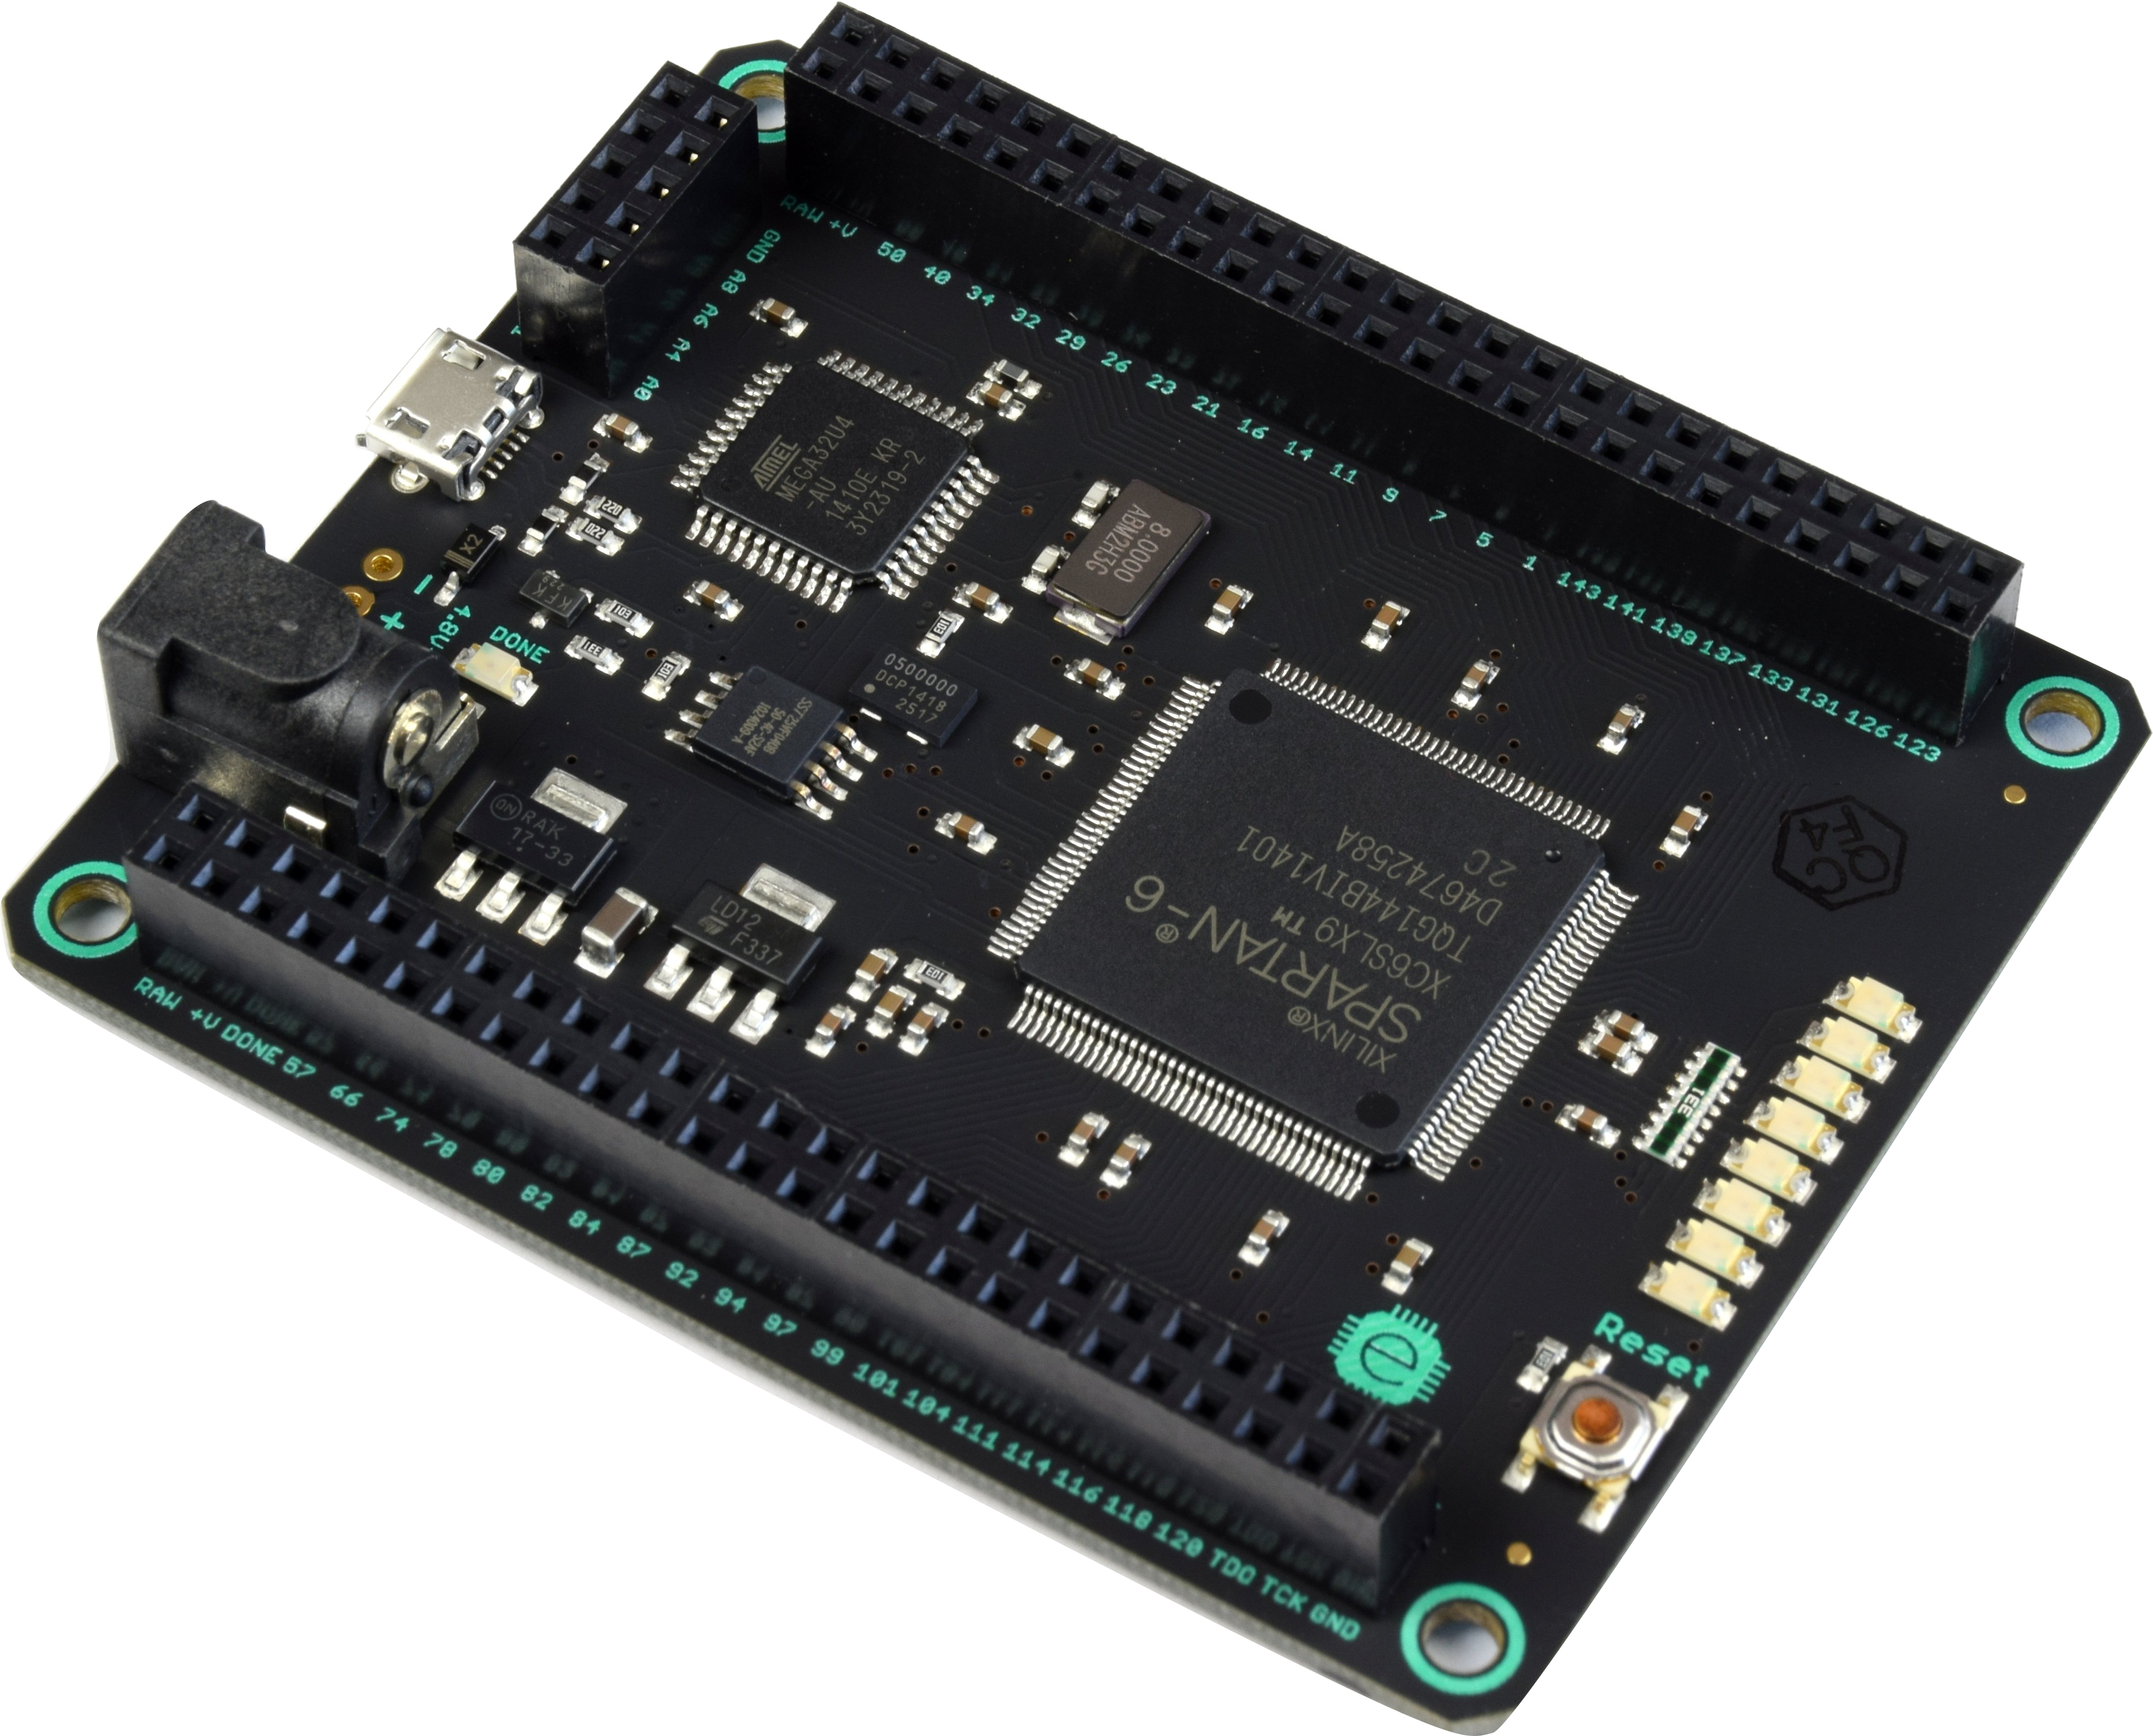
\includegraphics[width = 0.4\textwidth]{mojov3}
	\caption{Placa de prototipado rápido MOJO v3, diseñada por Embedded Micro}
	\label{mojo}
\end{figure}

La placa MOJO es una placa de desarrollo muy económica para prototipado, es decir, la fabricación de modelos funcionales. Para ello los puertos se disponen en un arreglo de pines a través de los cuales es posible acoplar el dispositivo que sea necesario. Se dispone en el mercado de otros circuitos impresos que se conectan a los pines y contienen un grupo de periféricos para propósito general. Estos impresos, se denominan shields ({\it escudo} traducido al castellano). se obtiene así una placa de desarrollo a la medida de las necesidades de cada proyecto. El usuario también puede diseñar sus shields o conectar las entradas y salidas de otros dispositivo mediante cables.%\\

Además de los shields, los diseñadores pensaron en que no sea necesario ninguna herramienta extra a la hora de programar la FPGA. Para ello, dotaron al sistema de un microcontrolador ATmega32U4 de Atmel con un programa de tipo bootloader, que se encarga de transferir la configuración del FPGA cargada desde una memoria flash incorporada, o trasmitida por el usuario desde una PC, a través de un transceptor USB que contiene el microcontrolador. Luego, el controlador es colocado en modo esclavo y se configura de forma tal que dota al sistema de una comunicación entre la FPGA y una PC, vía USB y se utiliza su ADC para leer los puertos analógicos.%\\%Luego, entra en modo esclavo, lo que permite al usuario, a posterior poder usar para debug el sistema USB que posee el microcontrolador.\\

Una vez llegado a este punto, el lector podría preguntar con toda razón ¿por qué es necesario realizar un sistema de comunicación USB extra, si ya cuenta con un microcontrolador que se encarga de dicho asunto? La respuesta se basa en el ancho de banda del sistema de comunicación que dispone la placa. La línea de controladores ATmega incorpora puertos USB 2.0 full-speed. Esto quiere decir que puede enviar datos a una tasa de \SI{12}{\mega\bit\per\second}. Además, la comunicación entre ambos chips se realiza via SPI (\(Serial Peripherical Interface\), o en español Interfaz Serie de Periféricos), comandada por un cristal de cuarzo de \SI{50}{\mega\hertz}, ofreciendo una velocidad de salida que puede resultar insuficiente a los fines de este trabajo. Se pretende dotar al sistema del mayor ancho de banda posible, utilizando la capacidad de USB 2.0 High-Speed, de hasta \SI{480}{\mega bp\second}.%\\

La placa de desarrollo Mojo fue seleccionada debido a su bajo costo, la versatilidad que ofrece y que está dotada por un Spartan-VI de Xilinx, que es un FPGA con una buena relación entre recursos, rendimiento, velocidad y precio.%\\